\documentclass[]{report}
\usepackage[hmargin=1.25in,vmargin=1in]{geometry} %调整页边距
% \usepackage[inner=1in,outer=1.25in]{geometry} %书籍左右不等宽排版
\usepackage[utf8]{inputenc}
\usepackage[]{ctex} %据说可以直接调用诸如 \kaishu \fangsong \heiti 的命令修改字体
\usepackage[svgnames]{xcolor} % Using colors
% \usepackage{background} % To include background images
\usepackage{fancyhdr} % Needed to define custom headers/footers
\usepackage[]{xeCJK}
\setCJKmainfont[BoldFont = STHeiti, ItalicFont = STKaiti]{Songti SC Light} %中文主字体
\setCJKsansfont[BoldFont = Weibei SC, ItalicFont = HanziPen SC]{Xingkai SC Light} %中文无衬线字体
\setCJKmonofont[BoldFont = Libian SC, ItalicFont = STFangsong]{Yuanti SC Light} %中文等宽字体
\setmainfont{Times New Roman} %\rmfamily
\setsansfont[ItalicFont = American Typewriter]{Comic Sans MS} %\sffamily
\setmonofont{Courier} %\ttfamily
\renewcommand{\emph}[1]{\textbf{\textit{#1}}}
\usepackage{titlesec}
\titleformat{\chapter}{\centering\huge\bfseries}{第~\thechapter~章}{1em}{}

\usepackage{ulem} %解决下划线、删除线之类的
\usepackage{listings}
\lstset{
language=C++,
keywordstyle = \color{blue}\bfseries,
commentstyle=\color{green},
tabsize = 4,
%backgroundcolor=\color{bg}
emph = {int,float,double,char},emphstyle=\color{cyan},
emph ={[2]const, typedef},emphstyle = {[2]\color{red}} }

\usepackage{amsmath} %数学公式问题
\usepackage{amsthm} %公式环境,如proof
\usepackage{booktabs} %三线表
\newcommand{\tabincell}[2]{\begin{tabular}{@{}#1@{}}#2\end{tabular}} %解决单元格内部换行的问题
% 比如这个 Beijing & 0,5 & 1,6 & 2,7 & 3,8 & 4,9 & The number changes every 3 months \\
% 改成这个 \tabincell{l}{Beijing}& \tabincell{c}{0,5}& \tabincell{c}{1,6}& \tabincell{c}{2,7}& \tabincell{c}{3,8}& \tabincell{c}{4,9}& \tabincell{c}{The number changes \\ every 3 months} \\
% 一个单元格过长,整行都需要修改
% 可以配合 \resizebox*{h-width}{v-width}{contents, e.g.tabular} 使用

\usepackage{mathrsfs} %在公式里面使用那个最花的字体
\usepackage{amssymb} %公式里面用空心黑体和旧式字体
\usepackage{amssymb} %AMS符号
\usepackage{amsthm} %AMS定理环境

\usepackage{markdown} %使用markdown语法,在编译时需要打开 shell-escape 标记,即 $ xelatex --shell-escape example.tex
\markdownSetup{hashEnumerators = true} %允许使用 #. 的方式编写有序列表
\markdownSetup{inlineFootnotes = true} %允许使用脚注形式的超链接,调用语法为 [anchor](uri), ^[footnote], <uri>
\markdownSetup{fencedCode = true} %以反引号和缩进来插入代码段,相当于 verbatim
\markdownSetup{
  pipeTables = true
} %支持表格的用法 (图片已经在markdown包里面支持了)
% \usepackage{booktabs} %解决三线表的线条粗细问题

\usepackage{graphicx} %插入图片
\usepackage{pdfpages} %插入PDF文件
\usepackage{makeidx}

\usepackage{tikz} %带圈字符
\usepackage{etoolbox} %带圈字符 (提供robustify)
\usepackage{enumitem}
\newcommand*{\circled}[1]{\lower.7ex\hbox{\tikz\draw (0pt, 0pt)%
    circle (.5em) node {\makebox[1em][c]{\small #1}};}} %新定义命令:带圈字符
\robustify{\circled}
% \usepackage{enumerate} %有序列表

\usepackage{hyperref} %超链接
% \usepackage[hidelinks]{hyperref} %隐藏超链接的红框
\markdownSetup{
  inlineFootnotes = true,
  renderers = {
    link = {\href{#3}{#1}},
  }
} % markdown块中使用直接点进去的超链接
% \setlist[enumerate,1]{label=(\arabic*).,font=\textup,leftmargin=7mm,labelsep=1.5mm,topsep=0mm,itemsep=-0.8mm}
% \setlist[enumerate,2]{label=(\alph*).,font=\textup,leftmargin=7mm,labelsep=1.5mm,topsep=-0.8mm,itemsep=-0.8mm}

\usepackage{braket}

%%%%%% Setting up the style

% \setlength\parindent{0pt} % Gets rid of all indentation
% \backgroundsetup{contents={\includegraphics[width=\textwidth]{ustc-name.pdf}},scale=0.4,placement=top,opacity=0.6,color=cyan,vshift=-20pt} %  USTC Logo

\pagestyle{fancy} % Enables the custom headers/footers

% Use default headers
% \lhead{} \rhead{} % Headers - all  empty

% \title{\vspace{-1.8cm}  \color{DarkRed} Laboratory Rotation Report}
% \subtitle{Title of the proposal % Title of the rotation project
% \vspace{-2cm} }
% \date{\today} % No date

\lfoot{\color{Grey} \textit{上官凝}}  % Write your name here
\rfoot{ \color{Grey} \texttt{\textit{操作系统原理与设计复习笔记}} }
\cfoot{\color{Grey} \thepage}

\renewcommand{\headrulewidth}{0.0pt} % No header rule
\renewcommand{\footrulewidth}{0.4pt} % Thin footer rule

\title{操作系统笔记}
\author{上官凝}
\date{\today}

\linespread{1.3} %行间距为1.3倍默认间距 (1.3 x 1.2倍字符宽度)

\makeindex

\begin{document}
\theoremstyle{definition} \newtheorem{theorem}{Thm}[section] %定义一个定理Thm,序号为section的下一级序号
\theoremstyle{definition} \newtheorem{definition}{Def}[section] %定义一个定义Def,序号为section的下一级序号
\theoremstyle{plain} \newtheorem{lemma}{lemma}[section] %引理

	\maketitle
	\newpage

	\tableofcontents
	\newpage

	\chapter{导语}
	\section{序幕}
	\textit{曾经有一位计算机学院的教授说过,计算机是文科。现在我信了。}\par
	建议多翻PPT,以及CS:APP。这门课的主题,正如PPT上所言(process lifecycle, process management, and other related issues are essential topics of this course),是围绕着进程来说的。注意每一个PPT的summary。\par
	OS和COD除去绪论,我认为都是一个由简单到复杂,不断发现异常、引入新理论解决异常的过程。不过很多时候最终的往往是做了tradeoff,比如内存不够的时候,可以用虚存。贴一张图\footnote{看到虚存那一页PPT就理解这个梗了233333}:\par
	\begin{figure}[h]
		\centering
		
\includegraphics[scale = 0.3]{images/Dream_World.jpg}
		\caption{Virtual Memory}
	\end{figure}
	\section{我愿意管他们叫定义}
	万一出个选择呢\par
	\begin{enumerate}
		\item The operating system contains the codes that are needed to work with the file system. The codes are called the kernel.
		\item “The one program running at all times on the computer” is the kernel.
		\item Kernel is the place where the system call implements.
		\item C is the only language to interact with the OS directly.
		\item Mechanisms determine \textit{\textbf{how}} to do something; policies determine \textit{\textbf{what}} will be done.
		\item If a process fails, most operating systems write the error information to a log file to alert system operators or users that the problem occurred. The operating system can also take a core dump.
		\item A process will switch its execution from user space to kernel space through invoking system call
		\item Windows maintains a forest-like hierarchy. (ch3 p39)
		\item A thread starts with one specific function. We name it the thread function. 其实就是说执行进程中的代码段,执行到某一句的时候,需要开线程了
		\item Critical sections is the code segment that is accessing the shared object, and it should be kept as tight as possible.
		\item A deadlock-free solution does not eliminate \textbf{starvation}
		\item 数据存储里面的一个缩写:BSS (Block Started by Symbol) Containing uninitialized global and static variables.
		\item A function can ask the CPU to read and to write anywhere in the stack, not just the “zone” belonging to the running function!
		\item 在虚拟内存分页的时候,Unallocated zone does not occupy any pages.
		\item Each process should have its own page table.
		\item If a process does not have enough frames – number of frames required to support pages in active use, frequent page fault would occur, replacing a page that will be needed again right away. This is called thrashing(抖动), spending more time paging than executing.
		\item Opening a file only involves the pathname and the attributes of the file, instead of the file content! A file descriptor returned.
		\item FAT 12/16/32: A block is named a cluster.
		\item GDT: group descriptor table (in Ext FS, ch10 part2 page 6)
		\item The number of files in the file system is fixed! Since\dots the inode bitmap has a fixed size.
		\item A hard link is a directory entry pointing to an existing file. Conceptually speaking, this creates a file with two pathnames. Thus increases the link count of that file.
		\item A symbolic link is a file. Unlike the hard link, a new inode is created for each symbolic link. It stores the pathname (shortcut). If the pathname is less than 60 characters, it is stored in the 12 direct block and the 3 indirect block pointers.
		\item A big-endian system stores the most significant byte of a word at the smallest memory address and the least significant byte at the largest.
	\end{enumerate}
	\section{我觉得比较重要的points}
	\begin{enumerate}
		\item 操作系统结构(ch2 page 45开始)
		\item 杂记(ch2 page 65开始)
		\item \verb|fork()|继承了什么(ch3 page 52, 53)
		\item 线程的参数传递(ch4 page 39)
		\item 多线程的进程,调用 \verb|fork()| 和 \verb|exec()|(ch4 page 55)
		\item UNIX 管道:\verb|fd[0]| 读端口 \verb|fd[1]| 写端口
		\item 进程间通信比较(ch5 page 44)
		\item 进程同步涉及到问题汇总(ch5 part2 page 24)
		\item 进程同步通信,race condition 及其解决(ch5 part2 page 31, 32)
		\item Entry \& Exit Section of Critical Section(ch5 part2 page 35, 36)
		\item 几种race condition的解决方案问题汇总(注意只要有busy waiting就会有优先权的问题)(ch5 part2 page 55)
		\item 信号量的命名:\verb|down(),P,wait()| 以及 \verb|up(),V,signal()|
		\item Deadlock Requirements(ch5 part2 page 7, 8)
		\item 对于死锁的判断:箭头指向圆圈表示这个实例已经分配给了圆圈里面的进程;箭头指向方框表示这个进程想要索取一个此资源的实例(ch5 part3 page 11)
		\item 处理死锁:银行家 (FSM?) 和鸵鸟
		\item 进程调度算法的优劣标准(ch6 page 30)注意有一个throughput指标:每时间段完成任务的进程数
		\item 数据段的内容(ch7 part1 page 14$\sim$24)
		\item 关于segmentation fault,可以看一下Wikipedia,以及(ch7 part1 page $78\sim85$)
		\item External Fragmentation \& Internal Fragmentation(ch7 part1 page 77)
		\item paging:虚拟内存的地址映射(ch7 part2 page 24)
		\item 分页一页是4kB,在page table里面,permission和Frame\#列,标有NIL的表示未分配,valid-invalid列表示这个虚拟页是否在内存里面(还可以在外存的……)
		\item TLB(caching的思想)(ch7 part2 page 42)
		\item 关于thrashing:为什么local replacement可以部分解决问题(可以避免踢出去别的进程的page);关于工作集working-set方案,当$\sum WSS_i>m$即所有进程的工作集加起来比可用的物理页框要多,就有可能会崩掉
		\item metadata元数据,见附件的Wikipedia,后面文件系统也会用到
		\item SSD的分级 package > die/chip > plane > block > page
		\item 特别注意SSD是不能overwrite的,只能program-erase-reprogram,有擦写寿命
		\item 在RAID那一块:MTTF(mean time to failure)
		\item RMW:利用旧的检验块和新旧修改块确定新的检验块,即读取旧的检验块和修改块;RRW:读取未改动块的数据
		\item open file table(ch9 part1 page 31)
		\item FS的3.0策略(ch9 part2 page 56 starts)注意 57页的block的definition
		\item metadata journaling两种模式(ch10 part2 page 70)
		\item TLB和大页表同时访问,所以计算所需时间的时候就 只会加上其中的一个
	\end{enumerate}

	\chapter{Mass Storage}
		\section{RAID}
		\begin{enumerate}
			\item Purpose :
			\begin{enumerate}
				\item In the past, combine small and cheap disks as a \emph{cost-effective} alternative to large and expensive disks
				\item  Nowadays
				\begin{enumerate}
					\item Higher performance
					\item Higher reliability via redundant data
					\item Larger storage capacity
				\end{enumerate}
			\end{enumerate}
			\item RAID-0: Block level stripping, no redundancy
			\item RAID-1: Data mirroring
			\item RAID-01: First stripping, then mirroring
			\item RAID-10: On the contrary of above
			\item RAID-4: Parity generation: Each parity block is the XOR value of the corresponding data disks $A_p=A_1\otimes A_2\otimes A_3$
			\begin{enumerate}
				\item RMW (read modify write) $A_p'=A_p\otimes A_1\otimes A_1'$
				\item RRW (read reconstruct write) $A_p'=A_3\otimes A_2'\otimes A_1'$
				\item Problem: \emph{Imbalance} -- Disk bandwidth are not fully utilized
				\begin{enumerate}
					\item Parity disk will not be accessed under normal mode
					\item Parity disk may become the bottleneck
				\end{enumerate}
			\end{enumerate}
			\item RAID-5: One parity per stripe
			\begin{enumerate}
				\item Key difference: Uniform parity distribution
			\end{enumerate}
			\item RAID-6: 2 parities
		\end{enumerate}

	\chapter{File System}
	\section{Programmer's perspective}
		\begin{enumerate}
			\item What are stored inside a storage device?
			\begin{enumerate}
				\item File
				\item Directories
				\item Interfaces/Operations
			\end{enumerate}
			\item Layout
			\begin{enumerate}
				\item what are stored inside the device
				\item Where the stored things are
				\item The set of FS operations defines how the OS should work with the FS layout. In other words, OS knows the FS layout and works with that layout.
			\end{enumerate}
			\item There are \emph{two basic things} that are stored inside a storage device, and are common to all existing file systems: File and Directories
			\item How does a FS store data into the disk? – That is, the \emph{layout} of file systems.
		\end{enumerate}
	\section{Why do we need files}
		\begin{enumerate}
			\item File provides a long-term information storage.
			\item File is also a shared object for processes to access concurrently.
			\item A unique pathname lead to the file's attributes and its content, which are usually stored \emph{separately}
		\end{enumerate}

		\subsection{File permissions}
		\begin{enumerate}
			\item \emph{First field:} File/director
			\item \emph{2nd} \emph{/3rd} \emph{/4th} \emph{fields (3 bits each):} controls read/write/execute
			\item for the file owner/file’s group/others (e.g., 111:7,110:6)
		\end{enumerate}

		\subsection{Opening a File}
		\begin{enumerate}
			\item The process supplies a path name to the OS.
			\item The OS looks for the \emph{file attributes} of the target file in the disk.
			\item The disk returns the file attributes.
			\item The OS then associates the attributes to a number and the number is called the \emph{file descriptor}.
			\item The OS returns the file descriptor to the process.
			\item Opening a file only involves the \emph{pathname} and the \emph{attributes of the file}, instead of the file content!
		\end{enumerate}

		\subsection{Read From Opened Files}
		\begin{enumerate}
			\item The process supplies a file descriptor to the OS.
			\begin{enumerate}
				\item A file descriptor is just an \emph{array index} for each process to locate its \emph{opened files}.
			\end{enumerate}
			\item The OS reads the file attributes and uses the stored attributes to \emph{locate the required data}. (In the OPEN FILE TABLE !)
			\item The disk returns the required data. -- File data is stored in a fixed size \emph{cache in the kernel}.
			\item The OS fills the \emph{buffer provided by the process} with the data. Write data to the userspace buffer.
		\end{enumerate}

		\subsection{Read System Call}
		\begin{enumerate}
			\item Check whether the end of the file is reached or not. [ Comparing \emph{size} and \emph{file seek}. ]
			\begin{enumerate}
				\item File attributs: Name, Identifier (\textit{Unique tag (a number which identifies the file within the FS)}), Type, Location, Size, Owner, Permission, Access, creation, modification time, etc.
				\item Runtime Attributes: reading position count, etc
			\end{enumerate}
			\item Reading data.
			\item File data is stored in a fixed size cache in the kernel.
			\item Write data to the userspace buffer.
		\end{enumerate}

		\subsection{Write System call}
		\begin{enumerate}
			\item Write data to the kernel buffer.
			\item According to the data length,
			\begin{enumerate}
				\item change in file size, if any (File attributes)
				\item change in the file seek (Runtime attributes)
			\end{enumerate}
			\item The call returns
			\item The buffered data will be flushed to the disk from time to time.
		\end{enumerate}
	\section{Directories}
		\begin{enumerate}
			\item It's a file
			\item Whether it has file attributes is FS-dependent
			\item It must have file content
		\end{enumerate}

		\subsection{Locate a File Using Pathname}
		\begin{quote}
			Suppose that the process wants to open the file \verb|/bin/ls|.
		\end{quote}
		\begin{enumerate}
			\item The process then supplies the OS the unique pathname \verb|/bin/ls|.
			\item The OS retrieves the directory file of the root directory \verb|/|.
			\item The disk returns the directory file.
			\item The OS looks for the name “bin” in the directory file.
			\item If found, then the OS retrieves the directory file of \verb|/bin| using the information of the file attributes of \verb|bin|.
			\item The OS looks for the name \verb|ls| in the directory file \verb|bin|. If found, then the OS knows that the file \verb|/bin/ls| is found, and it starts the previously-discussed procedures to open the file \verb|/bin/ls|
		\end{enumerate}

		\subsection{Creation and Deletion}
		\begin{enumerate}
			\item \emph{File creation == Update of the directory file}
			\begin{enumerate}
				\item \verb|touch text.txt| will only create the directory entry, and there is no allocation for the file content.
			\end{enumerate}
			\item Removing a file is just delete the information in Directory file.
			\begin{enumerate}
				\item Note that we are not ready to talk about de-allocation of the file content yet.
			\end{enumerate}
		\end{enumerate}
	\section{File System Layout}
		\subsection{Trial 1.0: The Contiguous Allocation}
		Just like a book! Yet drawbacks:
		\begin{enumerate}
			\item External Fragmentation (We have enough space, but there is no holes that I can satisfy the request.) Therefore we need to move files to clean up enough space.
			\item When a file need to grow, it may also do not have enough space.
			\item Used suitable for read-only cases
		\end{enumerate}

	\chapter{一些常见的题目}
	整理整理作业,得到一个cache,命中率还是可以很高哒
	\section{内存管理}
		\subsection{Segmentation Fault}
		段错误简单来说是由非法访问内存引起的,有三种(其实差不多的)说法:
		\begin{enumerate}
			\item When you are accessing a piece of memory that is not allowed to be accessed, then the OS returns you an error called –\ segmentation fault.
			\item (WikiPedia) In computing, a \emph{segmentation fault} (often shortened to \emph{segfault}) or \emph{access violation} is a fault, or failure condition, raised by hardware with memory protection, notifying an operating system (OS) the software has attempted to access a restricted area of memory (a memory access violation).
			\item The memory in a process is separated into \emph{segments}. So, when you visit a segment in an illegal way, then...\emph{segmentation fault}.
		\end{enumerate}\par
		下面这张图标有\textsf{\textit{YES}}的表示这种访问会引发段错误,标为\textsf{\textit{NO}}的不会引发
		\begin{figure}[h]
			\centering
			\begin{minipage}{40em}
				\centering
				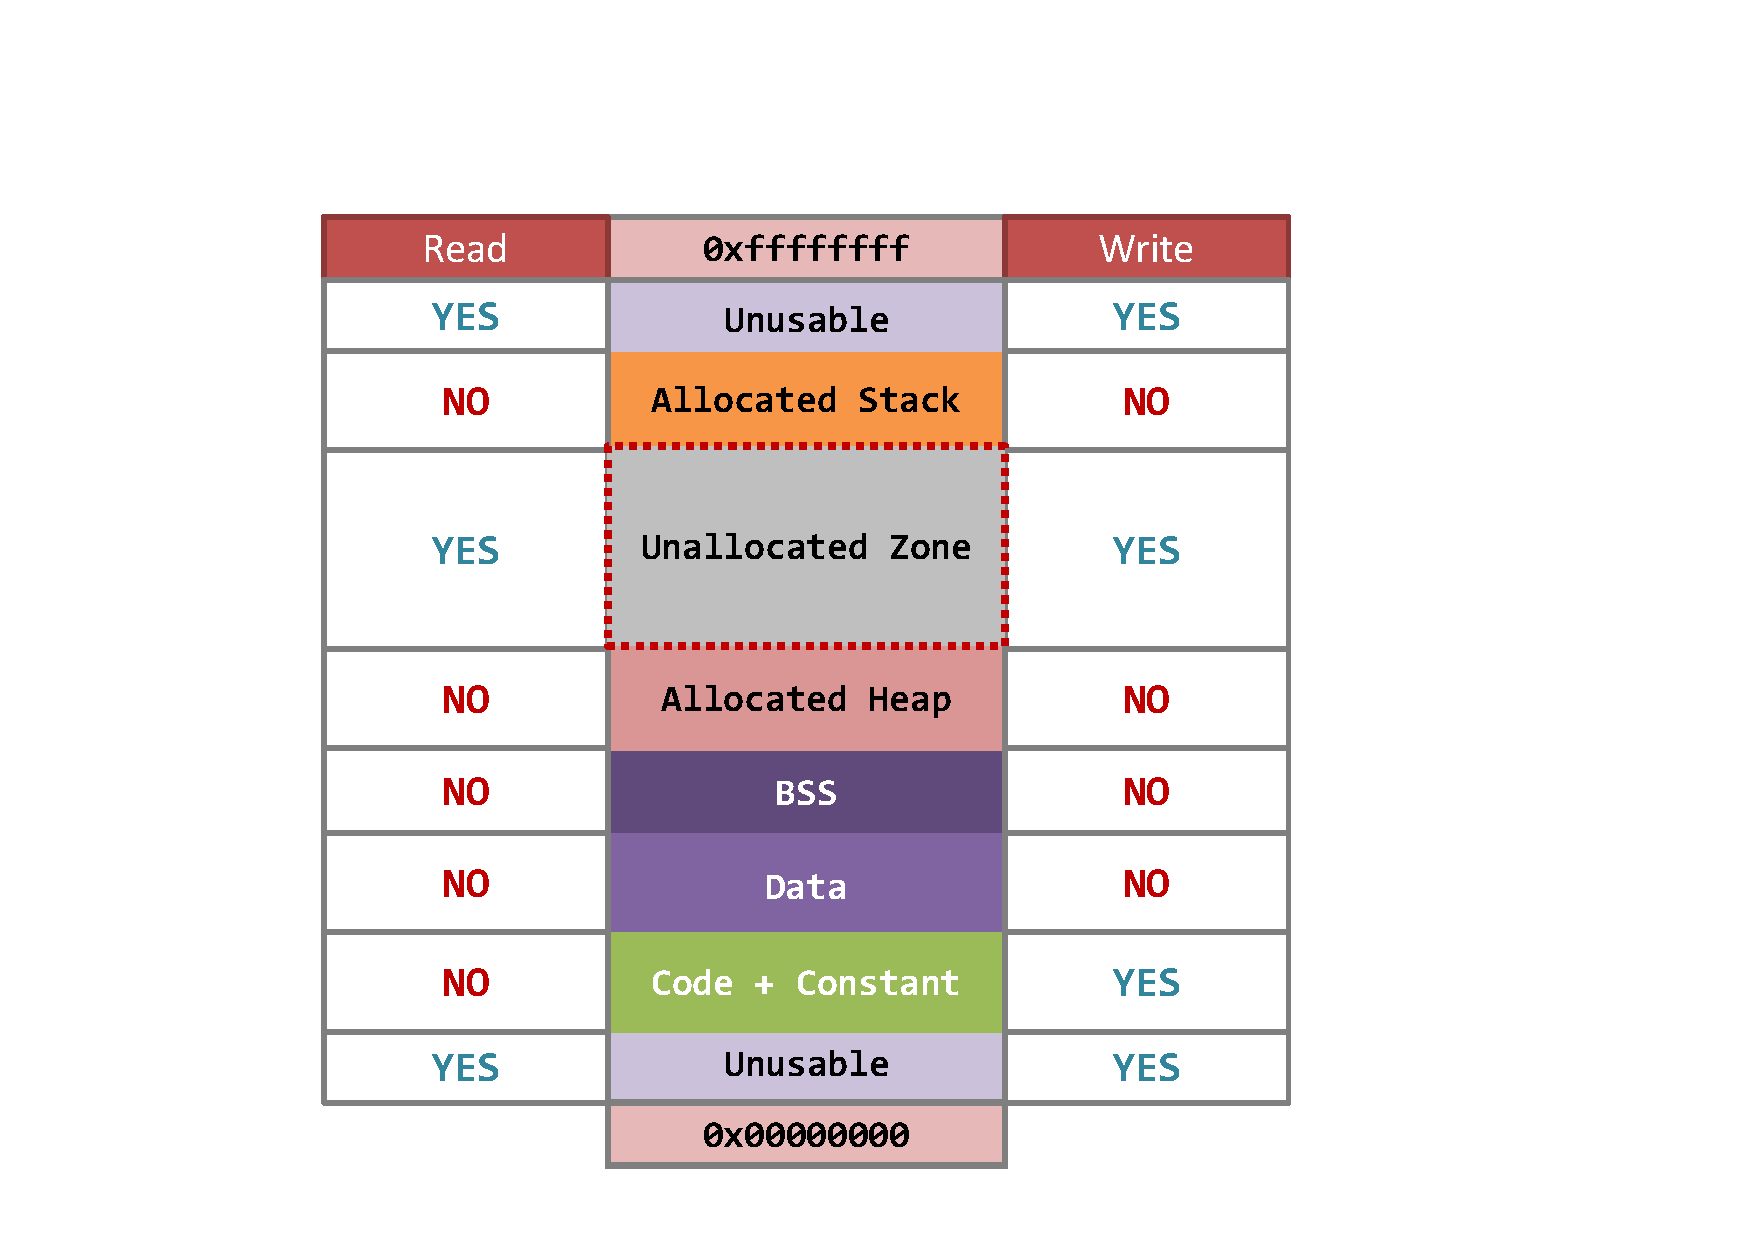
\includegraphics[scale = 0.4]{images/Segmentation_Fault.pdf}
				\caption{非法访问内存触发段错误的条件}
			\end{minipage}
		\end{figure}\par
		简单分一下类,可以这么看访问(代码+常数段是只读段;已分配的栈、堆、BSS (Block Started by Symbol)、数据段都是Allocated部分;栈从高地址向低地址长,堆相反,这两个会在中间遇上?):
		\begin{table}
			\centering
			\begin{tabular}{cccc}
				\toprule
				&\multicolumn{3}{c}{Segments to Visit}\\
				\cmidrule{2-4}
				&Read-only Segments&Allocated Segments&Unused or Unallocated Segments\\
				\midrule
				Reading&No Problem&No Problem&Segmentation Fault\\
				Writing&Segmentation Fault&No Problem&Segmentation Fault\\
				\bottomrule
			\end{tabular}
		\end{table}
	\section{文件系统}
		\subsection{FAT系统的读取流程}
		大致分为两步,即读取目录文件找到第一块的位置编号,和从FAT表链式遍历找到需要读取的块编号。FAT表里面存储了磁盘的content部分,各级文件(包括目录文件)所有文件的信息。其实查找一个cluster就是在一个array里面找到相应的hash关系。有两种找法:一个文件刚开始的位置,是在root directory里面,文件中间的是用FAT表来查找下一块的位置。\par
		\begin{figure}[h]
			\centering
			\begin{minipage}{20em}
				\centering
				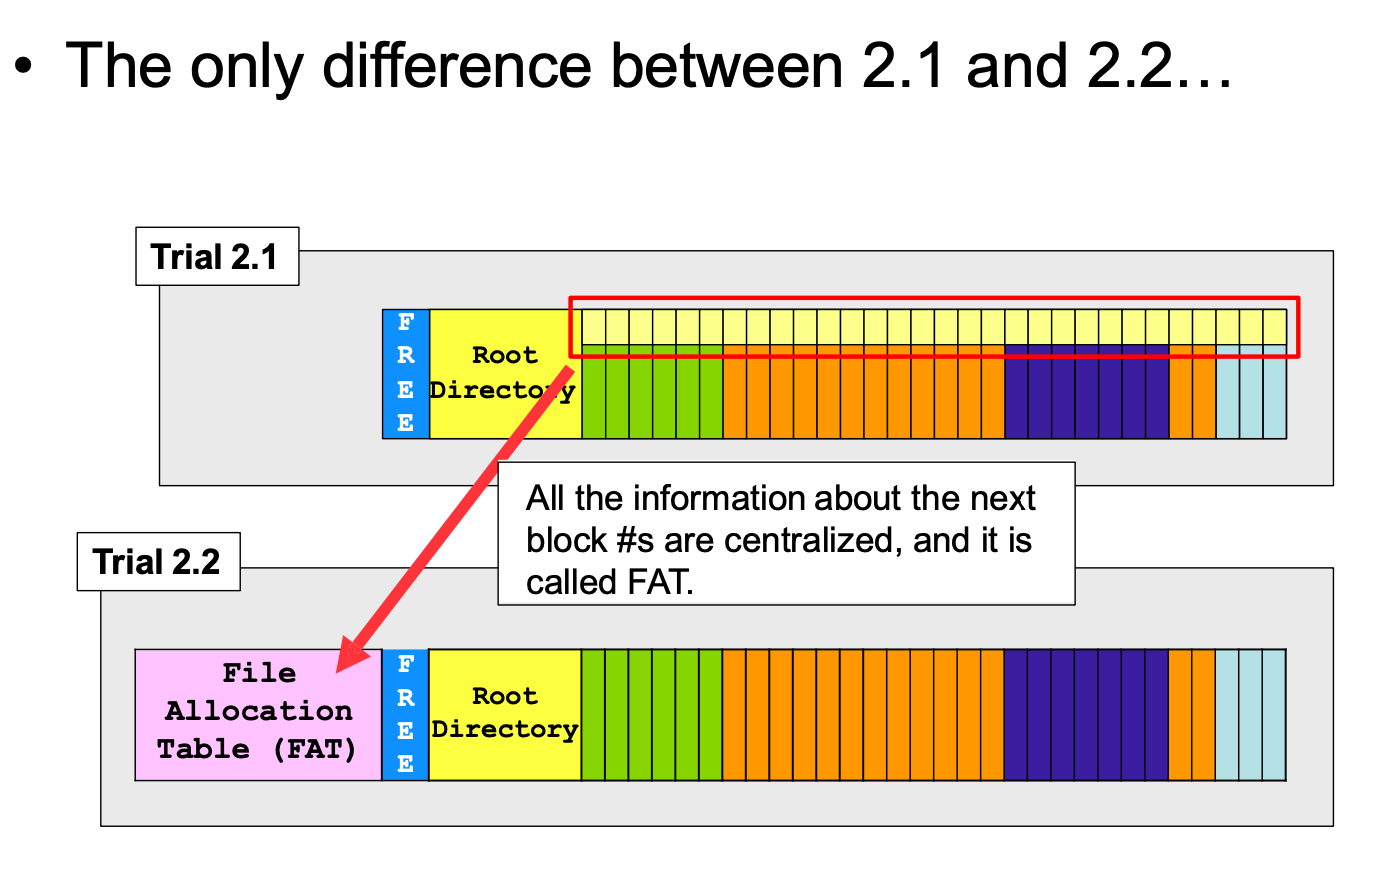
\includegraphics[scale = 0.15]{images/FAT.png}
				\caption{FAT Structure}
			\end{minipage}
			\begin{minipage}{20em}
				\centering
				\begin{minipage}{20em}
					\centering
					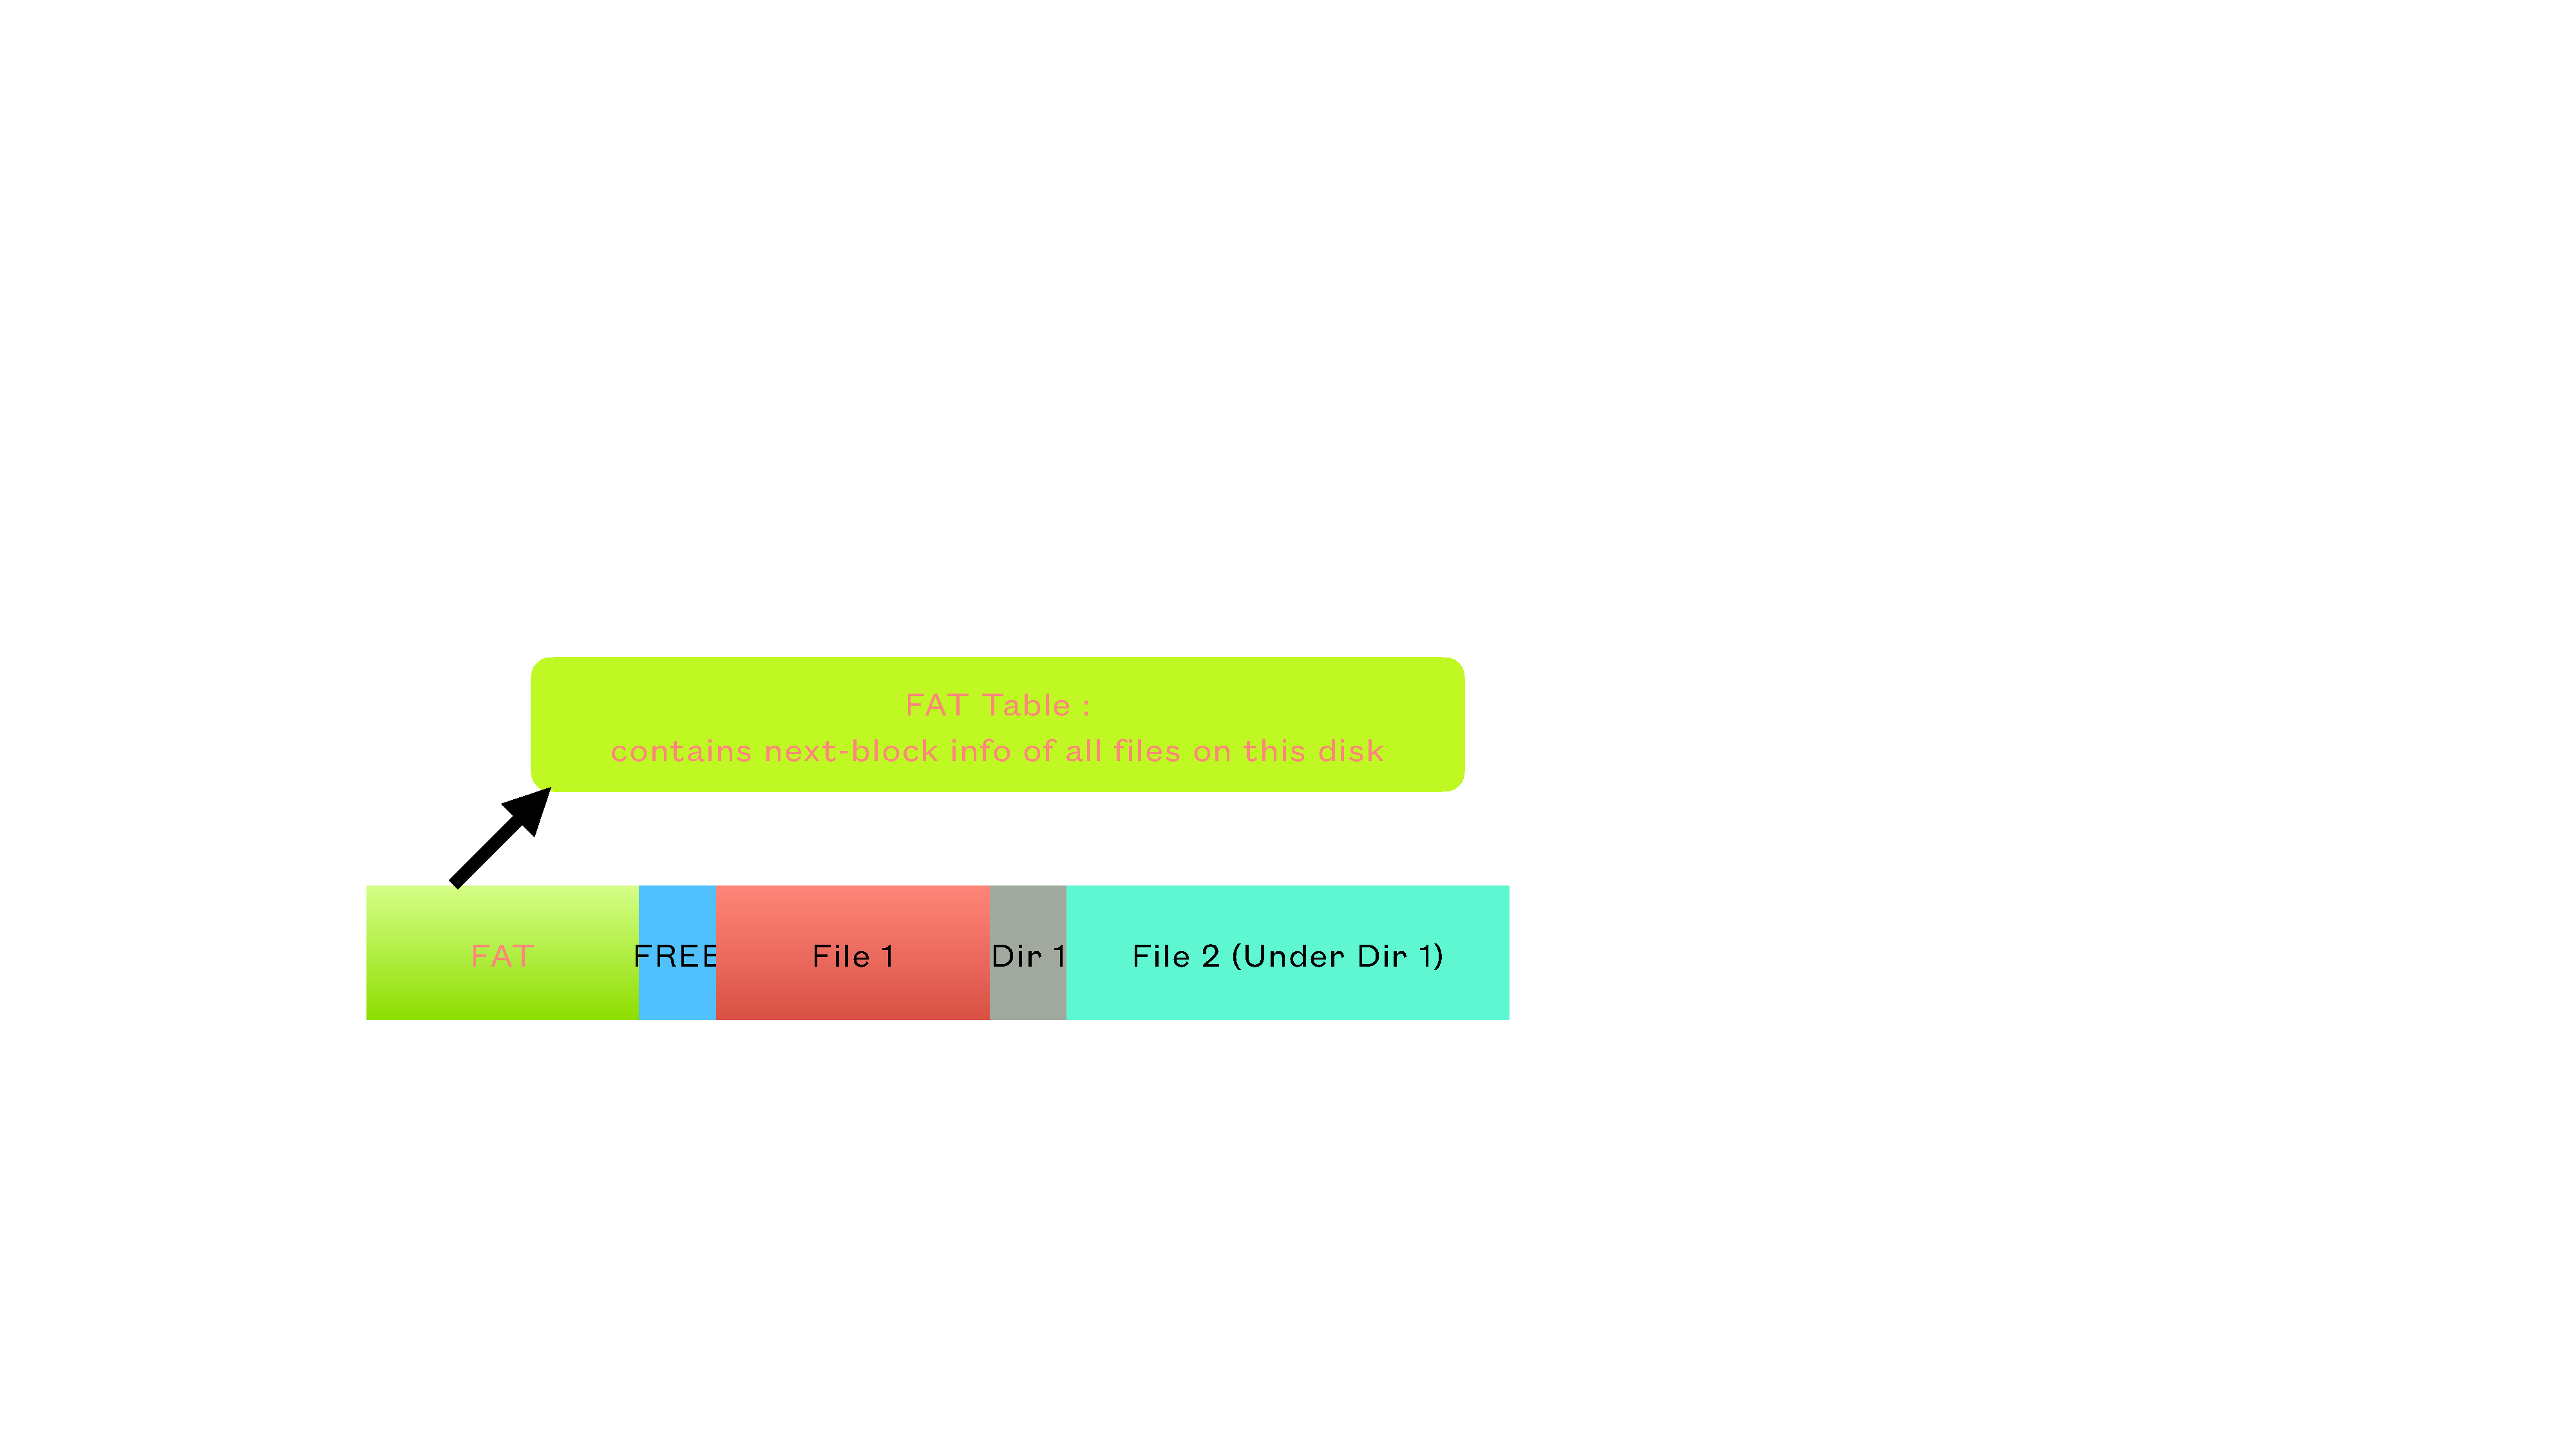
\includegraphics[scale = 0.18]{images/FAT_Explain_1.pdf}
					\caption{FAT表包含目录和多级文件}
				\end{minipage}
				\begin{minipage}{20em}
					\centering
					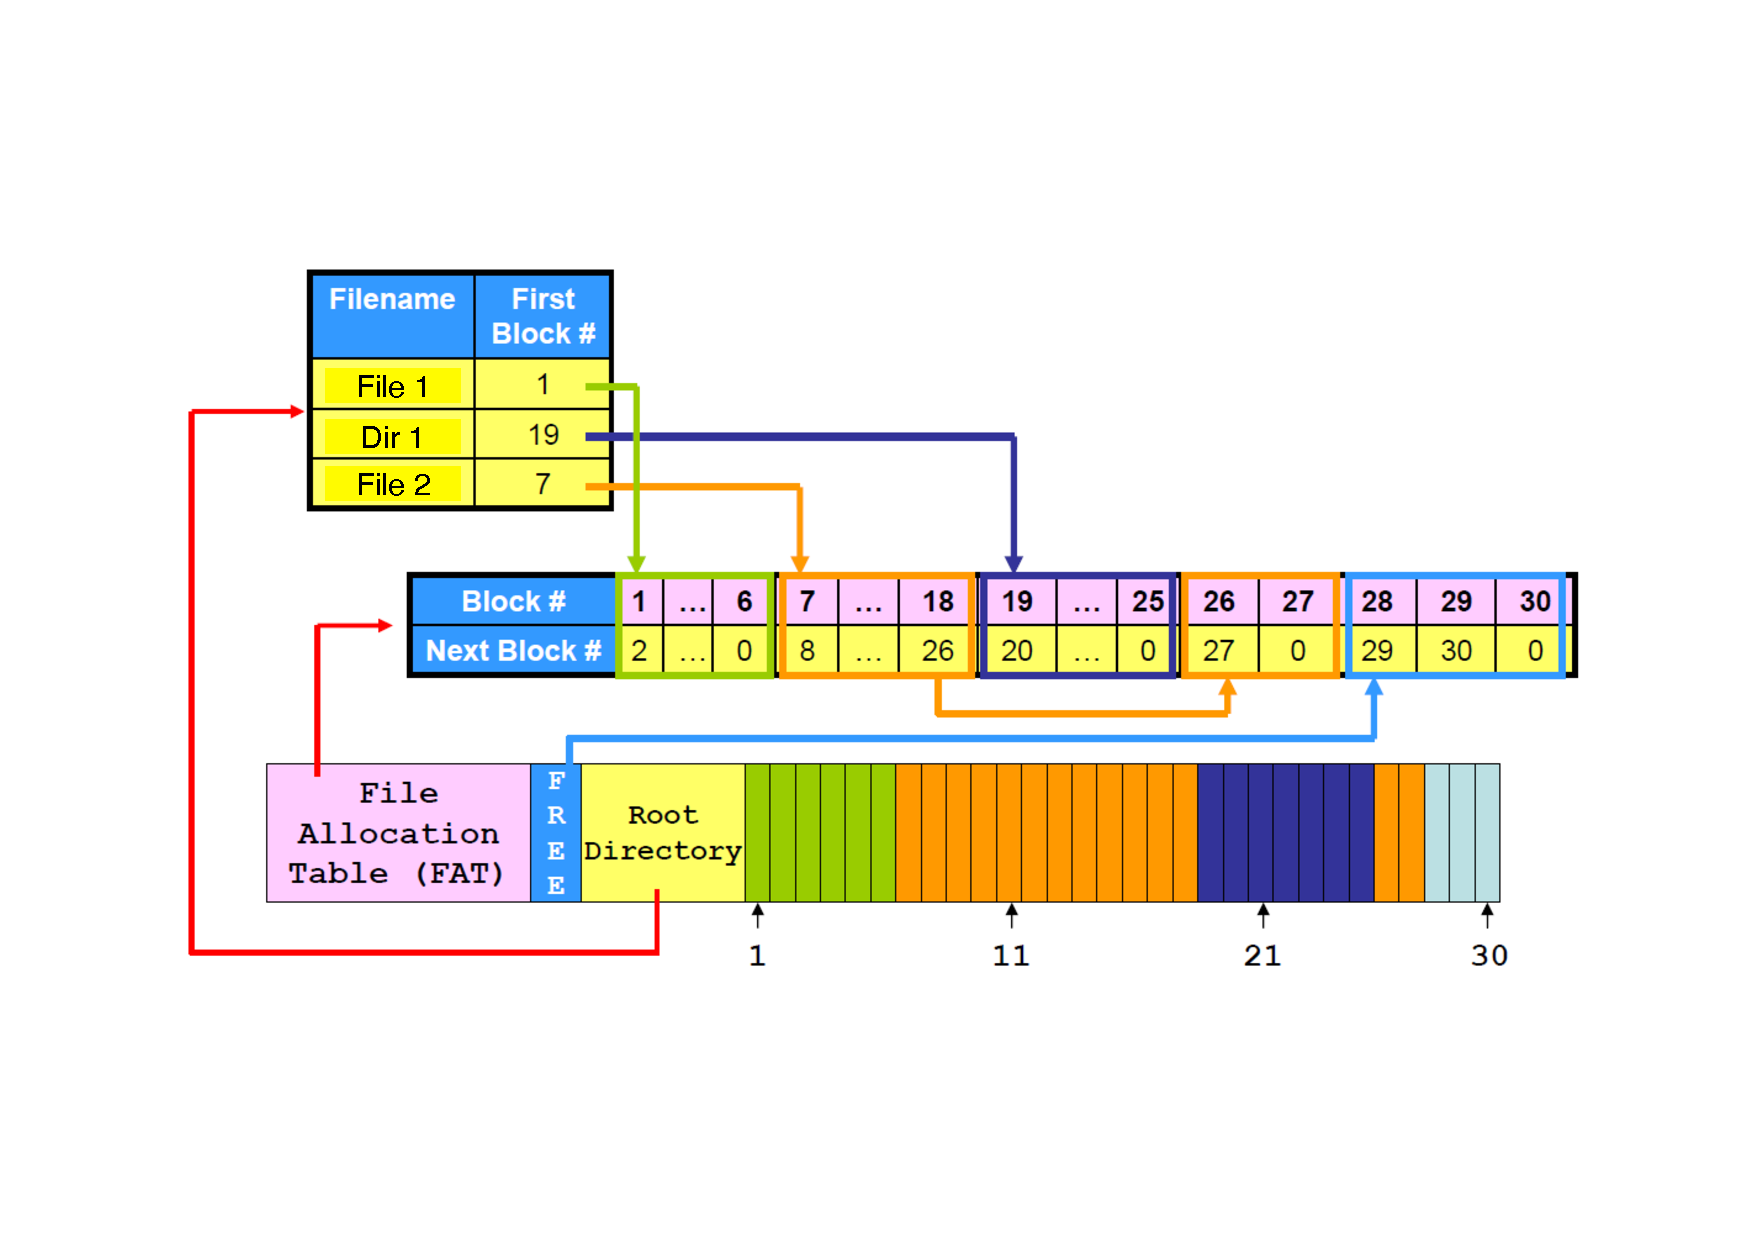
\includegraphics[scale = 0.23]{images/FAT_Explain_2.pdf}
					\caption{FAT表包含目录和多级文件}
				\end{minipage}
			\end{minipage}
		\end{figure}
		另外一个需要注意的是FAT表必须cache进kernel,至少一部分要被cache进去,否则依然解决不了random access效率很低的问题
		\subsection{Ext系统的读取流程}
		\paragraph{Inode的构建}
		回看一下FAT系统,效率上的亮点在于cache到kernel的FAT,但磁盘容量的增加会导致需要缓存的表变得很大。于是在Inode实现方案里面就不再缓存了(但是还是需要保存一个Open File Table的)。Ext一上来就先将FAT按照文件切开,每一个文件有一个自己的小FAT,构成一个结构体数组。这是为了解决FAT结构里面缓存不够灵活,导致性能和空间必须有很明显的Tradeoff的问题。为什么要用一个整齐的结构体数组呢,因为只有每一个Node的大小是一样的,才可以在从目录文件中查找得知目标文件的Inode编号的时候,计算出偏移量得到这个文件对应的Inode的具体位置。如果是变长Node,那么就像Trial 1.0一样,会面临外部碎片化的问题。而至于为什么这里就可以使用一个统一的结构来强制规范化对齐,而1.0就不可以,是因为Inode里面存的是元数据,比较小,这些内部碎片化就可以接受了。
		\begin{figure}[h]
			\centering
			\begin{minipage}{40em}
				\centering
				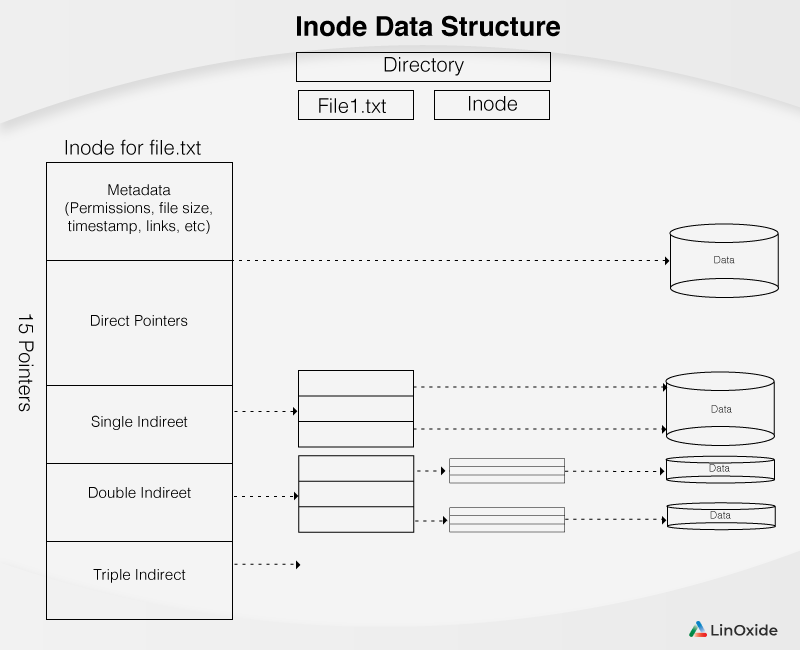
\includegraphics[scale = 0.3]{images/inode-data-structure.png}
				\caption{Index Node Structure}
			\end{minipage}
			\\[5pt]
			\begin{minipage}{40em}
				\centering
				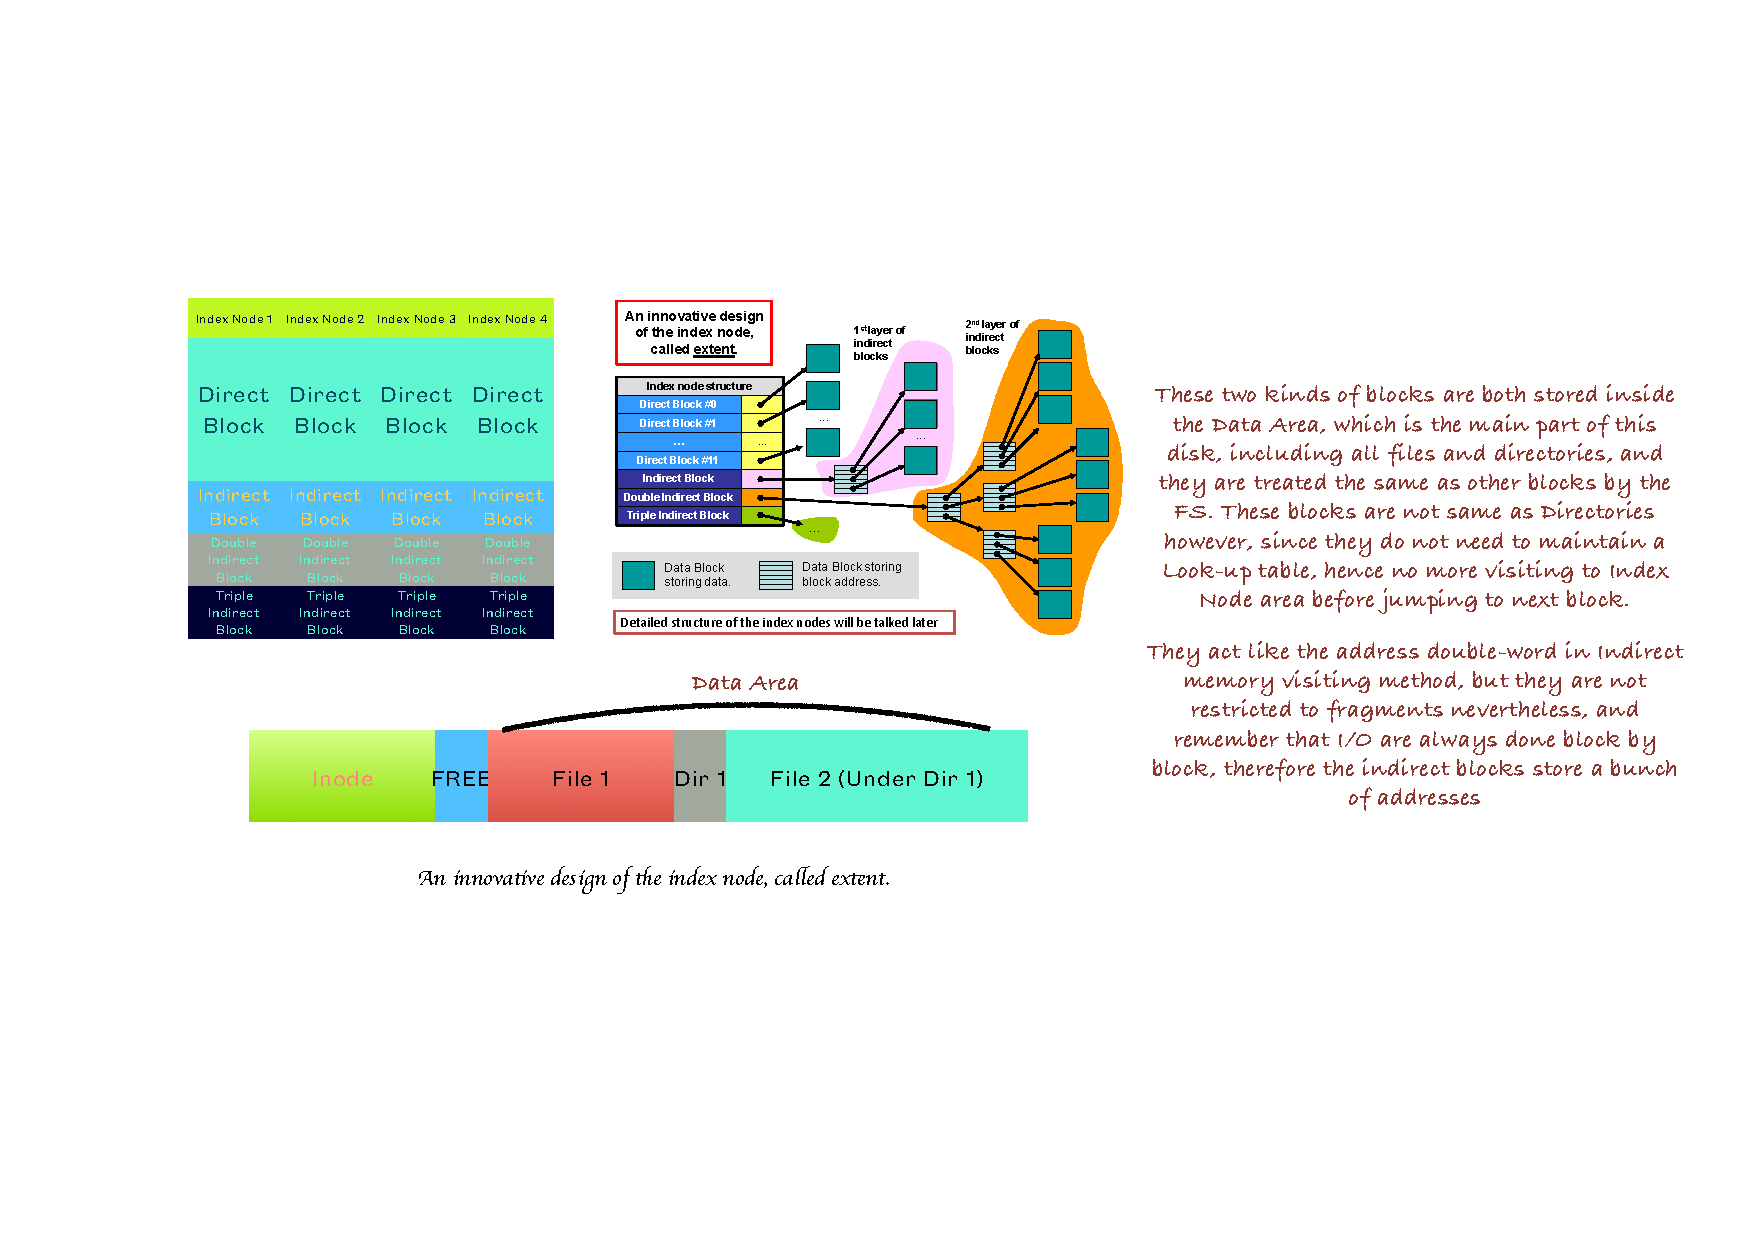
\includegraphics[scale = 0.57]{images/Inode_Structure.pdf}
				\caption{基于Inode的FS索引结构}
			\end{minipage}
		\end{figure}
\end{document}

